\documentclass{standalone}
\usepackage{tikz}
\usepackage{../mss}
\usepackage{sansmath}

\usetikzlibrary{shapes.geometric,positioning,calc,petri,graphs,fit,backgrounds}
\tikzset{
        node distance=1.35cm and 1.35cm,
        >=latex,
        font=\sf\bfseries\sansmath,
        ,
        every edge/.append style={line width=1.0pt}
        textfeld/.style={align=center,minimum height=0.5cm,minimum width=1.5cm},
        pfeil/.style={->,line width=1.0pt},
        box/.style={rectangle,draw,line width=1.0pt,minimum height=1.5cm,minimum width=2.8cm,align=center},
        place/.style={circle,line width=1.0pt,draw=black,minimum size=6mm},
        transition/.style={rectangle,line width=1.0pt,draw=black,minimum size=6mm},
        module/.style={rectangle,fill=gray!25,line width=1.0pt,inner sep=10pt},
        module label/.style={text=gray!90},
        synchronization/.style={draw,dashed,rounded corners,inner sep=6pt}
        }

\tikzgraphsset{
    every graph/.style = {use existing nodes}
}

\begin{document}
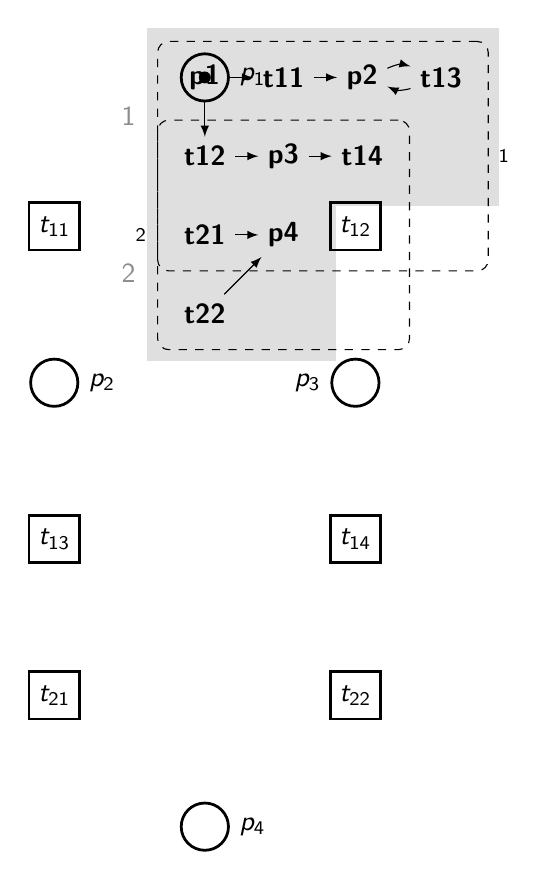
\begin{tikzpicture}

    \node[place,tokens=1,label=right:$ p_1 $] (p1) {};

    \node[transition] (t11) [below left=of p1] {$ t_{11} $};

    \node[transition] (t12) [below right=of p1] {$ t_{12} $};

    \node[place,label=right:$ p_2 $,below =of t11] (p2) {};

    \node[place,label=left:$ p_3 $,below =of t12] (p3) {};

    \node[transition] (t13) [below =of p2] {$ t_{13} $};

    \node[transition] (t14) [below =of p3] {$ t_{14} $};

    \node[transition] (t21) [below =of t13] {$ t_{21}$};

    \node[transition] (t22) [below =of t14] {$ t_{22} $};

    \coordinate(mid) at ($(t21)!0.5!(t22)$) ;

    \node[place,label=right:$ p_4 $] [below =of mid](p4) {};

    \graph{
    p1 -> t11 -> p2 ->[bend left=20] t13 ->[bend left=20] p2, p1 -> t12 -> p3 -> t14, t21 -> p4, t22 -> p4
    };

    % synchronizations
    \node[synchronization,
        fit=(t13)(t21),
        label={right:$ \synchronization_1 $}
    ]{};
    \node[synchronization,
        fit=(t14)(t22),
        label={left:$ \synchronization_2 $}
    ]{};

    % modules
    \begin{scope}[on background layer]

        \node[module,
            fit=(p1)(p2)(p3)(t11)(t12)(t13)(t14),
            label={[module label]left:$ \module{1} $}
        ] {};
        \node[module,
            fit=(p4)(t21)(t22),
            label={[module label]left:$ \module{2} $}
        ]{};
    \end{scope}

\end{tikzpicture}
\end{document}